\chapter{Implementation}\label{chapt:implement}

This chapter describes the implementation of the chosen test procedure and the related test parameter. Afterward, the results are presented and interpreted. The test procedure consists of the following stages:

% start item counter at zero
\begin{enumerate}\addtocounter{enumi}{-1}
    \itemsep-1.3em 
    \item Describe the workloads and parameters by which a system is to be tested.
    \item Test the unoptimized system using the specified workloads and parameters.
    \item Generate a weighted call graph from the workload on the unoptimised system.
    \item Sort the weighted call graph into a linear list using a function-ordering heuristic.
    \item Create a new optimised system using this linear list.
    \item Test the optimised system using the specified workloads and parameters.
\end{enumerate}

An Intel Core i3-6100U CPU with skylake microarchitecture is used as the test processor. This model features a 4KiB ITLB and DTLB with 64 entries and a shared 4KiB second level TLB with 1536 entries. Furthermore, each core has its own L1 data cache, L1 instruction cache and L2 cache. The L3 cache is shared between all cores. \cite{cpuinfo} 

The implementation is based on the performance analyse tool \textit{perf}, which is readily available in the kernel. The complete implementation can be found at \cite{github}, while simplified code snippets can be found in chapter \ref{appendix:implement}.

\vspace{-\baselineskip}

\section{Workload}

\enlargethispage{2\baselineskip}
For the implementation of the workloads, it is important that these predominantly affect functionality in the kernel space, i.e. they need to be kernel centric. This means that rather than CPU intensive workloads which run mostly in user space, there will be workloads that focus on stressing kernel tasks like network, scheduler, filesystem, etc.

That said, the objective is not to optimise the whole kernel but rather subsystems of it because there is functionality in the kernel where optimization is not useful for the performance, such as for example the \textit{debugfs} filesystem.

In order to avoid possible causes of interference, it is advisable to interact as little as possible with external components. For example, in workloads like databases which involve heavy disk I/O operations, the workload will be I/O-bound. This means the measurement will include the time taken for data transfers between the disk and the system, thus diverting the focus away from kernel centric tasks.

Furthermore, to create a more realistic workload scenario, it was decided to run the workload on a Linux operating system with a desktop environment. At the time of writing, the latest stable version of Debian bullseye was used as the base. This approach helps to create a more accurate end result, as it mimics a more real world environment for the workload, thus providing a clearer recommendation for the use of code collocation in the kernel for an end user. The disadvantage of this, however, is that other causes and effects of interference can creep in and blur the results of the analysis.

For this thesis a network driven workload was chosen. An attempt was made to implement a database workload, but it did not demonstrate the same degree of precise repeatability as a network workload. Furthermore, it is important to ensure that the workload is sufficiently intense during runtime to overshadow other processes running in user space which could also access the kernel space at the runtime of the workload. This can be achieved with an increased workload priority and an increased number of workload processes.

Furthermore, one could fine-tune parameters for the network workload in order to achieve a more frequent traversal of the network code in kernel space. For example, the \textit{direct memory access (DMA) ring buffer} could be set to the minimum for the used network card.

\enlargethispage{3\baselineskip}
This fine-tuning option is used in this thesis for the call stack analysis, but not for the analysis of the PMU events. The reason is that in the call stack analysis, it is important to create as precise a weighted call graph as possible. The higher precision result, which is acquired from the frequent traversal of the code, then affects the function-sorting heuristic as well as the final linear list. However, for the actual workload test where the PMU events are analysed, it is important to expose them to more real-world circumstances. Since most people do not change these parameters but use the default values, there could be a risk of blurring the final result of the analysis.

\section{PMU events}\label{section:events}

The selection of the PMU events strongly determine the interpretation of the results and must therefore be carefully chosen. As different processor models may have different PMU events implemented, it is important to select those that provide a more concrete interpretation of the objective.

% In addition, one should note that ITLB misses are caused by an instruction fetch, which happen primarily in the frontend of the pipeline.
In this thesis, the aim is to reduce ITLB pressure, so PMU events were chosen to measure the number of ITLB misses, CPU stalls, or page table walks during the runtime of the workload. The following PMU events from \cite{skylake_events}, with the help of  \cite[p. 266]{brendan} and \cite{propeller}, were chosen for the used processor model:

\begin{itemize}
    \item \spcstring{ITLB_MISSES.MISS_CAUSES_A_WALK}\\
    "Counts page walks of any page size (4K/2M/4M/1G) caused by a code fetch. This implies it missed in the ITLB and further levels of TLB, but the walk need not have completed." \cite{skylake_events}
    \item \spcstring{ITLB_MISSES.WALK_ACTIVE}\\
    "Cycles when at least one [Page Miss Handler] is busy with a page walk for code (instruction fetch) request. [Extended Page Table] page walk duration are excluded in Skylake microarchitecture." \cite{skylake_events}
    \item \spcstring{ITLB_MISSES.WALK_COMPLETED}\\
    "Counts completed page walks (all page sizes) caused by a code fetch. This implies it missed in the ITLB (Instruction TLB) and further levels of TLB. The page walk can end with or without a fault." \cite{skylake_events}
    \item \spcstring{FRONTEND_RETIRED.ITLB_MISS}\\
    "Counts retired Instructions that experienced iTLB (Instruction TLB) true miss." \cite{skylake_events}
    \item \spcstring{ICACHE_64B.IFTAG_MISS}\\
    "Instruction fetch tag lookups that miss in the instruction cache (L1I). Counts at 64-byte cache-line granularity." \cite{skylake_events}
\end{itemize}

The distinction between retired instructions and code or instruction fetch must be taken into consideration. The PMU events described here could also count code or instruction fetches that were loaded and executed via speculative execution. \cite[p. 34-35, 46]{patmc} \cite{intel_retired}
\enlargethispage{\baselineskip}

This means that if an instruction loaded by the speculative execution is not needed, because for example the prediction was wrong, this instruction will be not retired and consequently flushed, i.e. the instruction will be not written back. Retired instructions are therefore instructions which are correctly predicted and successfully written back. \cite[p. 46]{patmc} \cite{intel_retired}

Intel has published a white paper on the subject of reducing ITLB miss stalls, which can be found at \cite{intel_opt_runtime}. They define metrics which can be also used in this thesis:

\begin{itemize}
    \item ITLB Stall Metric\\
    "This metric represents the fraction of cycles the CPU was stalled due to instruction TLB misses." \cite{intel_opt_runtime}
    \begin{align*}
        ITLB\_Miss_{stall} = 100 \cdot 
        \left( \frac{\spcstring{ICACHE_64B.IFTAG_STALL}}{\spcstring{CPU_CLK_UNHALTED.THREAD}} \right)
    \end{align*}
    \item  ITLB Misses Per Kilo Instructions (MPKI)\\
    "This metric is a normalization of the ITLB misses against number of instructions, and it allows comparison between different systems." \cite{intel_opt_runtime}
    \begin{align*}
        ITLB\_MPKI = 1000 \cdot \left( \frac{\spcstring{ITLB_MISSES.WALK_COMPLETED}}{\spcstring{INST_RETIRED.ANY}} \right)
    \end{align*}
\end{itemize}

PMU events can be used in two modes: counting and sampling. Counting mode is used to count the total number of occurrences of specific events within a certain time period, while sampling mode saves the instruction pointer at the time of the occurrence of the event. \cite[p. 55-56, 59-60]{patmc} \cite[p. 157-158]{brendan} In this thesis, counting mode will be used to check for a significant change in the selected events. It is important to note that the total number of events counted in a certain time period may vary depending on the system's state.
\vspace{-\baselineskip}

\section{Call stack analysis}

% Honorable mentions:
% https://easyperf.net/blog/2019/02/09/Top-Down-performance-analysis-methodology
% https://easyperf.net/blog/2019/08/02/Perf-measurement-environment-on-Linux#8-use-statistical-methods-to-process-measurements
% https://www.intel.com/content/www/us/en/docs/vtune-profiler/cookbook/2023-1/top-down-microarchitecture-analysis-method.html
% https://github.com/intel/perfmon

The chapter \ref{chapt:callgraph} serves as a basis for creating a weighted call graph for a specific workload. Although the creation of a weighted call graph can be done by static analysis, it is not recommended. Therefore, the weighted call graph will be analysed dynamically.

In order to obtain a realistic result, the overhead should be as minimal as possible, which is why profiling is used instead of tracing. To generate a call graph \textit{perf} supports the collection of call stacks, which captures the call stack at the time of the occurrence of the event. With the addition of a stack unwinder a call graph can be created out of the collected call stacks. \cite[p. 62]{patmc} \cite{stack-unwinder} 

A hardware feature which is recommended in several papers, projects and articles for the collection of call stacks is the \textit{last branch recording} (LBR) which further decreases the overhead of profiling. \cite{codestitcher, bolt, propeller, lwn-lbr} LBR uses model specific registers to store the last taken branches. \cite{easyperf-lbr} \cite{lwn-lbr} The LBR feature is in combination with \textit{perf} only supported for user call chains and not kernel call chains. \cite{man-perf-record}

The PMU event to be sampled on can be either \textit{cycles} or \textit{instructions}. However, \textit{cycles} is recommended because "empirically we found it to produce better results". \cite{llvm-bolt} It is also recommended by \cite{brendan-perf} to sample at an odd frequency of, for example 99Hz, instead of 100Hz to avoid locksteping. In addition, in this thesis the call graph will not be generated from profiling specifically the workload, but it will be generated from a system-wide profiling of the kernel space for each CPU. This has the advantage of capturing the entire system's execution, including interactions between different processes and threads. 

To further enhance the creation of call graphs, the used processor has a built-in  hardware feature called \textit{hardware event-based sampling} (EBS) and \textit{processor or precise event-based sampling} (PEBS). \cite[p. 158]{brendan}

EBS does not interrupt the process each time the event occurs, but only when the associated counter overflows, at which point the instruction pointer is collected. \cite[p. 59-60]{patmc} \cite{brendan-perf} The advantage of not collecting a sample for each interrupt but waiting for an overflow is the reduction in overhead and collected data size. Since it is not of interest which instruction pointer is present for every CPU cycle, the total number of information and the number of saved and to be evaluated samples can be reduced. With a large enough sample size, if the program is executed long enough, the results are as statistically important as without EBS. \cite[p. 59-60]{patmc} \cite{brendan-perf} \cite{intel_ebs}

Nevertheless, there is a risk of a possible delay between the event overflow and the collection of the instruction pointer with EBS, which results in recording an incorrect instruction pointer at the time of the overflow. The result is a wrong recording of the code line which has caused the overflow. This inaccuracy is called \textit{skid}. A hardware feature which the used processor implements to combat skid is PEBS. \cite[p. 158]{brendan} \cite{intel_skid}
\enlargethispage{\baselineskip}

Both the \textit{BOLT} project \cite{llvm-bolt} and the \textit{Propeller} project \cite{llvm-propeller} use the EBS functionality, but without PEBS. Whether the usage of the PEBS functionality will create a more precise weighted call graph is not known.

\section{Function ordering and compilation}

In order to evaluate the collected call stacks and create a linear list for the compilation, the raw data must be first converted into usable information for the function-sorting heuristic, i.e. into a weighted call graph. An example weighted call graph can be seen in figure \ref{fig:excallgraph}.

\begin{figure}[H]
    \centering
    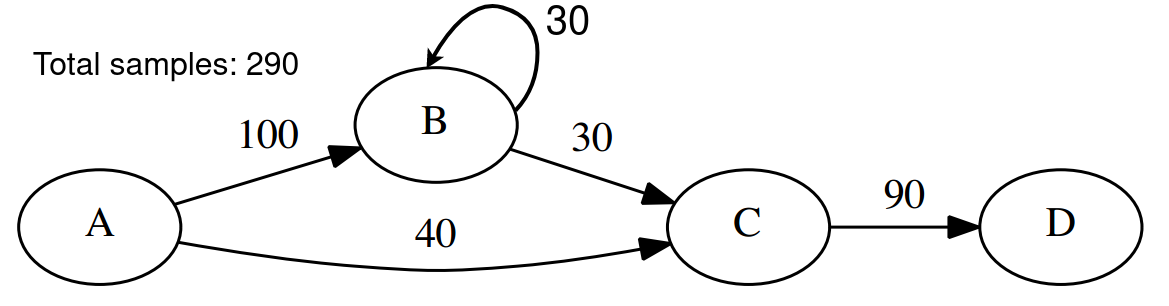
\includegraphics[width=.7\textwidth]{images/5_implementation/c3-custom-example.png}
    \caption{Modified example of a weighted call graph\\Source: \cite{hfsort}}
    \label{fig:excallgraph}
    \vspace{-\baselineskip}
\end{figure}

The parameters which are needed for the function-sorting heuristic can be acquired via an included raw data parser implementation of \textit{perf}. With this, important parameters such as unique caller-callee calls and the number of calls during the duration of the running system can be determined from the collected call stacks. Although \textit{perf} provides its own implementation interface for direct access to the raw data, this thesis has chosen to use the included implementation to obtain the necessary information.

Unfortunately, the included implementation of \textit{perf} creates cyclic node information, i.e. information which describes that a node calls itself. In the figure \ref{fig:excallgraph} an example can be seen where the node \textit{B} calls itself.  These samples can occur through, for example, recursive functions. This thesis considers cyclic nodes as part of the weighted call graph and includes them in the function-sorting heuristic accordingly. Any symbol names, i.e. function names, that were not obtained from the collected function pointers are sorted out.

\newpage

The function-sorting heuristic used in this thesis is the C3 heuristic because it offers better performance results than the PH heuristic. To implement the C3 heuristic, a weighted call graph and the function size of each individual function are required. This information can be obtained with \textit{perf}. The function size can alternatively be obtained via the generated \textit{System.map} file during the kernel compilation or via the \textit{kallsyms} functionality of the executed kernel.

For the C3 heuristic, it is also assumed that the total time spent in a node is equal to the sum of the incoming arcs. Accordingly, a cyclic node is included in the calculation of the total time of a node or the density of the individual clusters. A page size of 4KiB is specified, although other page sizes are possible.

The original authors have already implemented the C3 heuristic in the \textit{hfsort} utility, which is part of the \textit{hhvm} project \cite{hhvm}. This implementation generates a linear list from the weighted call graph, which can be used in the linker phase of compilation. To move individual sections, i.e. individual functions, in the linker phase, the kernel must be compiled with the compilation flag \textit{-ffunction-sections}.